\documentclass[11pt,a4paper]{article}
\usepackage[utf8]{inputenc}
\usepackage[T1]{fontenc}
\usepackage[spanish,es-nodecimaldot]{babel}
\usepackage{lmodern,amsmath,amssymb,graphicx,booktabs,float,xcolor,caption}
\usepackage[margin=2.2cm]{geometry}
\usepackage{url}
\makeatletter\g@addto@macro{\UrlBreaks}{\do\-\do\_\do\.}\makeatother
\urlstyle{tt}\DeclareRobustCommand{\archivo}[1]{\path{#1}}
\usepackage[colorlinks=true,linkcolor=blue!50!black,urlcolor=blue!50!black]{hyperref}
\captionsetup{font=small,labelfont=bf}
\graphicspath{{../figuras/}}
\newcommand{\aviso}[1]{\par\smallskip\noindent\fcolorbox{orange!70!black}{orange!8}{\parbox{\dimexpr\linewidth-2\fboxsep-2\fboxrule}{\small #1}}\par\smallskip}

\title{Corridas MEIGA con la fuente $^{241}$Am-Be: comparación de medios\\
\large y escalado al montaje blindado (373\,272 neutrones en 5 minutos)}
\author{Jaime Betancourt}
\date{20 de octubre de 2026}

\begin{document}
\maketitle

\begin{abstract}
Se recuperaron del disco TOSHIBA tres corridas de MEIGA con la fuente $^{241}$Am-Be: agua pura, 2.5\,\%
y 10\,\% NaCl, con 1\,637\,458 neutrones cada una. Los neutrones se inyectaron verticalmente \emph{por la
tapa} del tanque. Se compararon los tres medios y cada evento se reponderó por su energía inicial para
pasar del espectro sesgado del archivo de entrada al espectro ISO~8529. Con agua + 10\,\% NaCl, por
neutrón incidente, la eficiencia de señal ($Q\geq1$) sube de 36.4\,\% a 49.4\,\% y la carga media de
3.54 a 11.16~p.e.; las capturas en $^{35}$Cl pasan a ser el 67\,\%. Para el montaje
blindado (haz 35\,\% / halo 45\,\% / fondo 20\,\%), el haz se escaló con estas corridas y el halo y el fondo
con la respuesta monoenergética de la Campaña~1, que usa la misma inyección por la tapa. En 5~minutos se
esperan 88\,287 (agua pura), 107\,258 (2.5\,\%) y 136\,065 (10\,\%) eventos con señal.
Los resultados valen para inyección por la tapa; el montaje real irradia por el costado.
\end{abstract}
\tableofcontents

\section{Corridas recuperadas}
El archivo \archivo{Simulacion-fuente-241AmBe.zip} (TOSHIBA, 178~GB) se extrajo en
\archivo{ADATA HD330/Simulacion-fuente-241AmBe/}: 178 archivos (504.5~GB), todos con el
CRC verificado. Se omitieron dos zip internos que son copias de carpetas ya incluidas. Según el registro de MEIGA
(\archivo{Flujo-AmBe241-*.txt}), las tres corridas tienen la misma configuración:
\begin{itemize}
\item Entrada: \archivo{Espectro-completo-neutrones-fuente-AmBe241.txt} completo (1\,637\,458 neutrones), el archivo analizado en el informe de la fuente: 437 energías discretas, con el sesgo por la densidad de puntos digitalizados.
\item Inyección \texttt{eCircle}: disco de radio 0.2~m a $z=1.5$~m, en vertical hacia abajo, que entra por la tapa del tanque ($R=48$~cm, $H=133$~cm).
\item Geant4 10.7.p4, \texttt{QGSP\_BERT\_HP} sin S($\alpha,\beta$), detector \texttt{eSaltyWCD} con \texttt{impuritiesFraction} 0, 0.025 y 0.1.
\item Agua pura: solo se conservan \archivo{output.json} (carga por evento) y archivos procesados de gammas y electrones; los archivos de pasos no están. 2.5\,\% y 10\,\%: datos completos (\archivo{rastreo-neutron-completo.txt}, \archivo{neutrones-capturados.txt}, \archivo{secondary-particles-neutron-capturado.txt}, etc.).
\end{itemize}

\paragraph{Procesamiento.} \archivo{scripts/extraer_carga.py} lee la carga y la energía inicial de cada
evento en \archivo{output.json}. \archivo{scripts/procesar_pasos.sh} resume cada evento del archivo de
pasos de neutrones (un evento empieza en la traza 1, paso 1, e incluye los neutrones secundarios). Las
capturas por evento suman exactamente las líneas de \archivo{neutrones-capturados.txt} (1\,002\,377 y
1\,082\,920). El núcleo de cada captura se toma del residuo registrado en la misma posición: no queda
ninguna captura sin núcleo. El orden y la energía de los eventos coinciden entre \archivo{output.json} y
los archivos de pasos.

\paragraph{Reponderación al espectro ISO.} A cada una de las 437 energías $E_j$ (con $n_j$ eventos) se le
asigna la probabilidad ISO~8529 de su celda, delimitada por los puntos medios con sus vecinas, y cada evento
recibe el peso $w_j=P_\text{ISO}(\text{celda}_j)/(n_j/N)$. La energía media pasa de 4.064 a
4.211~MeV, igual a la del ISO digitalizado (4.211~MeV), con un número efectivo de eventos de
1\,331\,899 (Fig.~\ref{fig:rep}).

\begin{figure}[H]\centering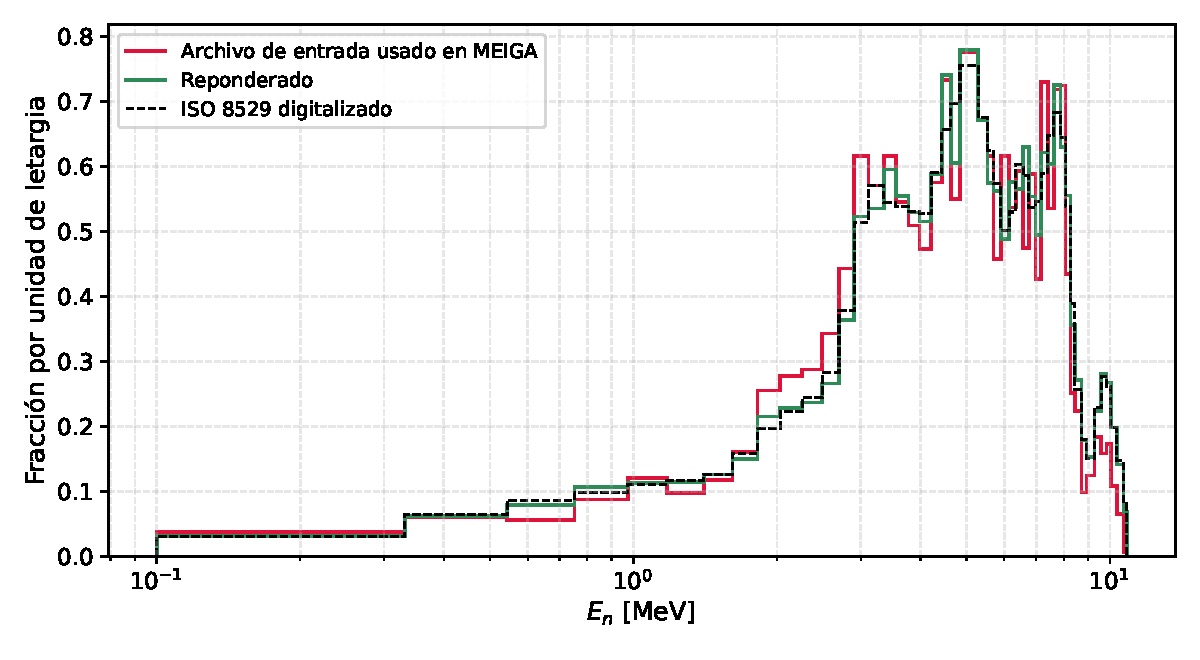
\includegraphics[width=0.72\linewidth]{fig06_reponderacion.pdf}
\caption{Espectro de los neutrones simulados (rojo), tras la reponderación (verde) y espectro ISO 8529 (negro).}\label{fig:rep}\end{figure}

\section{Comparación de los tres medios}
\begin{table}[H]\centering\small
\caption{Resultados por neutrón incidente. ``Archivo'': espectro simulado tal cual; ``ISO'': reponderado.
$^\dagger$Agua pura: sin archivos de pasos; $\eta_\text{cap}$ estimada (\S\ref{sec:etapura}).}\label{tab:medios}
\begin{tabular}{lccc}\toprule
 & Agua pura & Agua + 2.5\,\% NaCl & Agua + 10\,\% NaCl \\\midrule
$\varepsilon(Q\geq1)$ archivo [\%] & 36.13 & 41.88 & 49.12 \\
$\varepsilon(Q\geq1)$ ISO [\%] & 36.44 & 42.16 & 49.38 \\
$\varepsilon(Q\geq3)$ ISO [\%] & 17.99 & 27.31 & 37.78 \\
$\varepsilon(Q\geq20)$ ISO [\%] & 0.303 & 3.957 & 8.070 \\
$\langle Q\,|\,Q\geq1\rangle$ ISO [p.e.] & 3.54 & 7.79 & 11.16 \\
$\eta_\text{cap}$ archivo [\%] & --- & 61.22 & 66.13 \\
$\eta_\text{cap}$ ISO [\%] & 56.9$\pm$2.6$^\dagger$ & 61.25 & 66.16 \\
Capturas por neutrón (ISO) & --- & 0.6125 & 0.6616 \\
$P(\text{señal}\,|\,\text{captura})$ [\%] & --- & 66.2 & 71.9 \\
$P(\text{señal}\,|\,\text{sin captura})$ [\%] & --- & 3.7 & 4.7 \\
Capturas en H [\%] & 100 & 63.7 & 31.2 \\
Capturas en $^{35}$Cl / $^{37}$Cl [\%] & --- & 35.5 / 0.11 & 67.4 / 0.22 \\
Capturas en $^{23}$Na [\%] & --- & 0.58 & 1.11 \\
Gammas por captura & --- & 1.65 & 2.25 \\
Profundidad de captura, mediana [cm] & --- & 9.4 & 9.6 \\
Colisiones elásticas hasta la captura & --- & 80 & 53 \\
Primario: escapa / captura / inelástica [\%] & --- & 31.1 / 59.7 / 9.2 & 26.6 / 63.6 / 9.8 \\
\bottomrule\end{tabular}\end{table}

\begin{figure}[H]\centering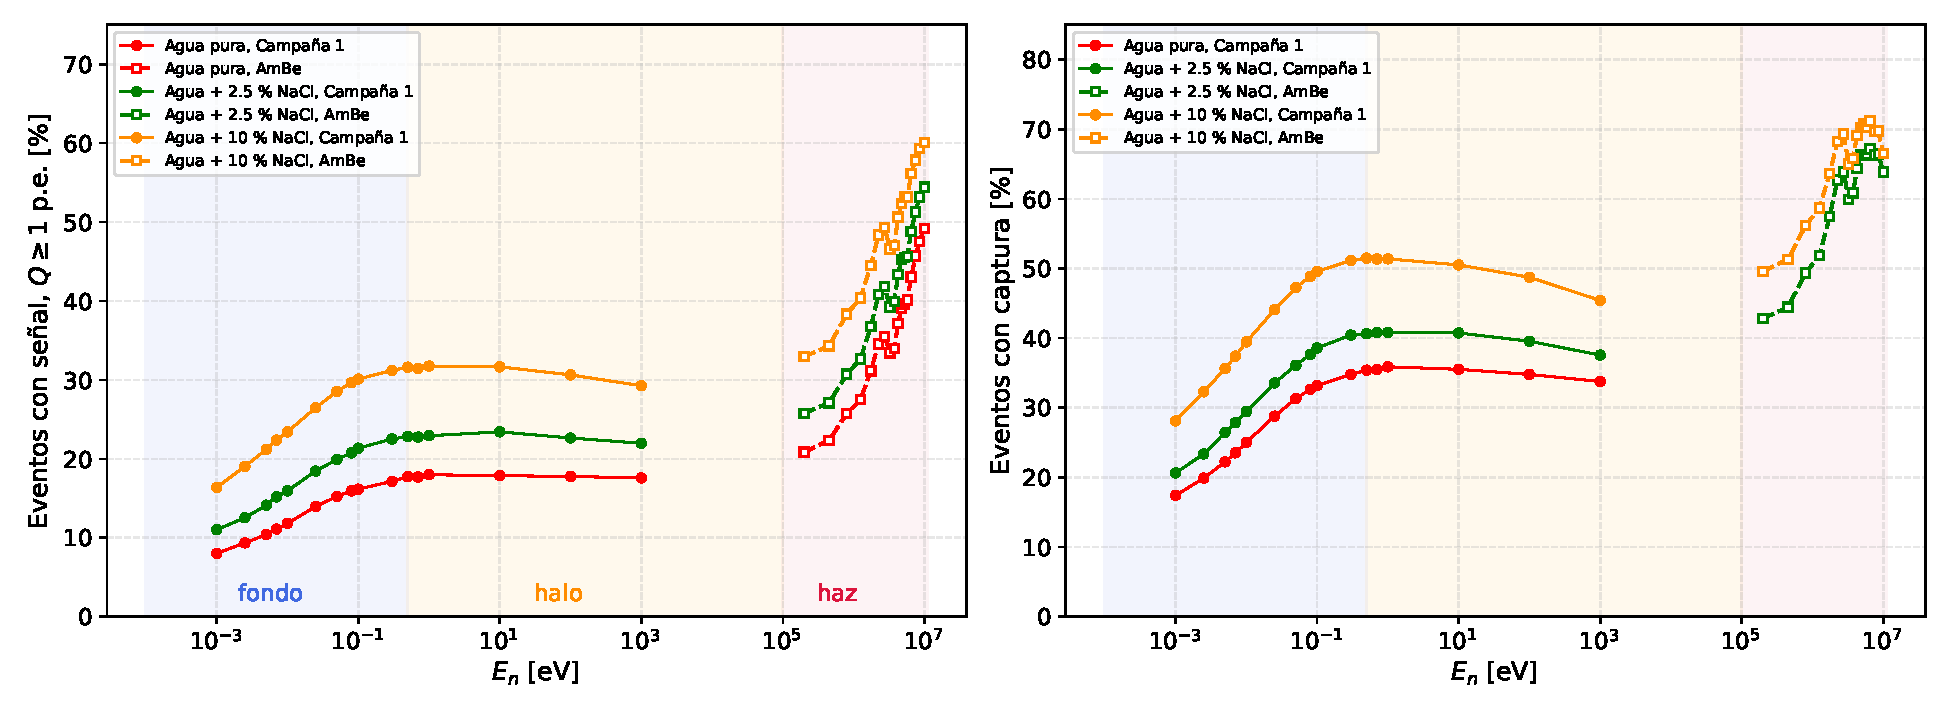
\includegraphics[width=\linewidth]{fig01_respuesta_vs_energia.pdf}
\caption{Eficiencia de señal y fracción de eventos con captura frente a la energía del neutrón: Campaña~1 (puntos llenos, 1~meV--1~keV) y corridas Am-Be en bandas de energía inicial (cuadros abiertos). Bandas de color: rangos del fondo, el halo y el haz del montaje blindado.}\label{fig:resp}\end{figure}

\begin{itemize}
\item \textbf{La reponderación cambia poco.} La eficiencia sube 0.3--0.4 puntos y la carga media menos del 2\,\%: la respuesta varía suavemente con $E$ entre 1 y 10~MeV, así que el sesgo de energía del archivo apenas se nota en estos observables.
\item \textbf{Efecto del NaCl.} Frente a agua pura, la eficiencia $Q\geq1$ sube un factor 1.16 (2.5\,\%) y 1.36 (10\,\%). Las señales grandes ($Q\geq20$) suben $\times$13 y $\times$27: las cascadas del $^{36}$Cl (8.58~MeV) producen más luz que el gamma de 2.224~MeV del hidrógeno.
\item \textbf{Coherencia con la Campaña~1.} La carga media de los eventos con señal (3.54 / 7.79 / 11.16~p.e.) es parecida a la de la Campaña~1 a 1~eV--1~keV (3.17 / 7.47 / 10.58~p.e.): la luz por captura no depende de la energía inicial. Por eso tiene sentido combinar las dos campañas en el escalado.
\item \textbf{Neutrones rápidos.} Con inyección por la tapa, se capturan más que los térmicos (61--66\,\% frente a 35--48\,\%): un neutrón de unos MeV penetra ~10~cm antes de termalizarse (mediana de profundidad ~9.5~cm, Fig.~\ref{fig:nuc}) y tiene menos probabilidad de volver a salir por la tapa. Además, el 9--10\,\% de los primarios sufre una interacción inelástica, que aporta gammas de desexcitación y explica que $P(\text{señal}\,|\,\text{sin captura})\approx4$--5\,\%.
\item \textbf{Núcleo de captura.} La fracción en $^{35}$Cl (35.5 y 67.4\,\%) coincide con la de las corridas de 500~MeV (35.8 y 67.7\,\%), y se repite el exceso de la línea de 8.58~MeV ya identificado en G4NeutronHP (Fig.~\ref{fig:gam}).
\end{itemize}

\begin{figure}[H]\centering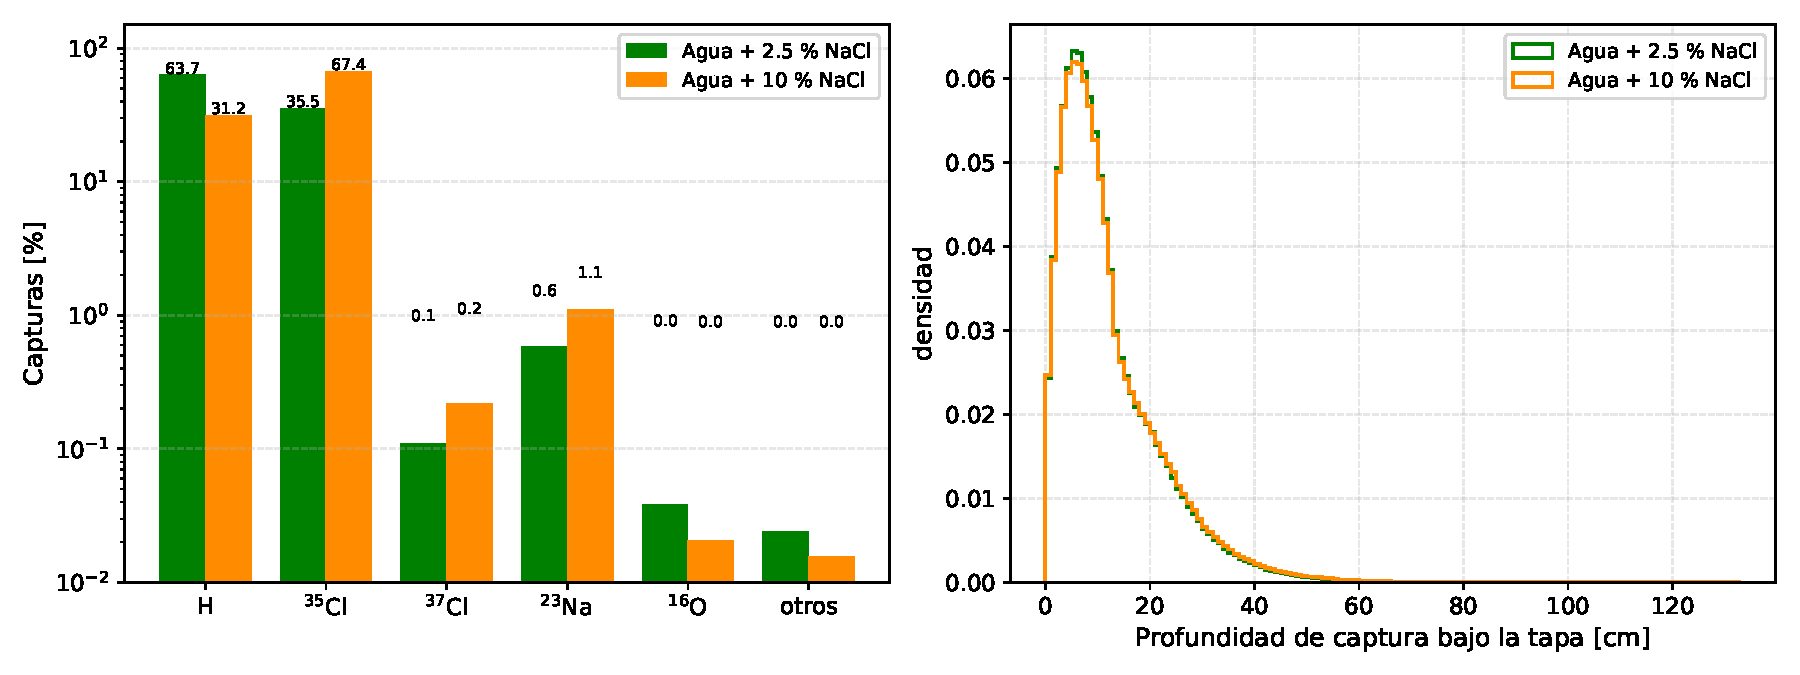
\includegraphics[width=\linewidth]{fig03_nucleo_profundidad.pdf}
\caption{Núcleo de captura y profundidad de captura del neutrón primario bajo la tapa (NaCl).}\label{fig:nuc}\end{figure}
\begin{figure}[H]\centering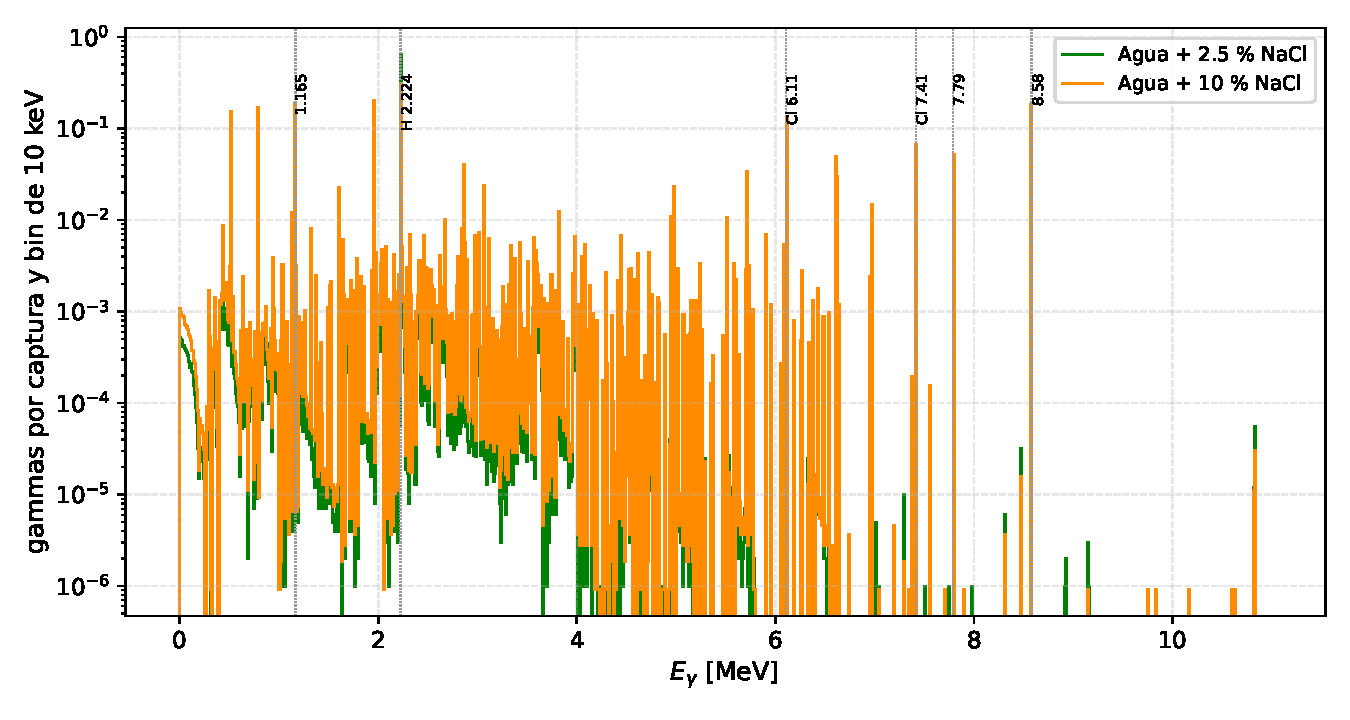
\includegraphics[width=0.85\linewidth]{fig04_gammas_captura.pdf}
\caption{Energía inicial de los gammas de captura (por captura, bins de 10~keV).}\label{fig:gam}\end{figure}
\begin{figure}[H]\centering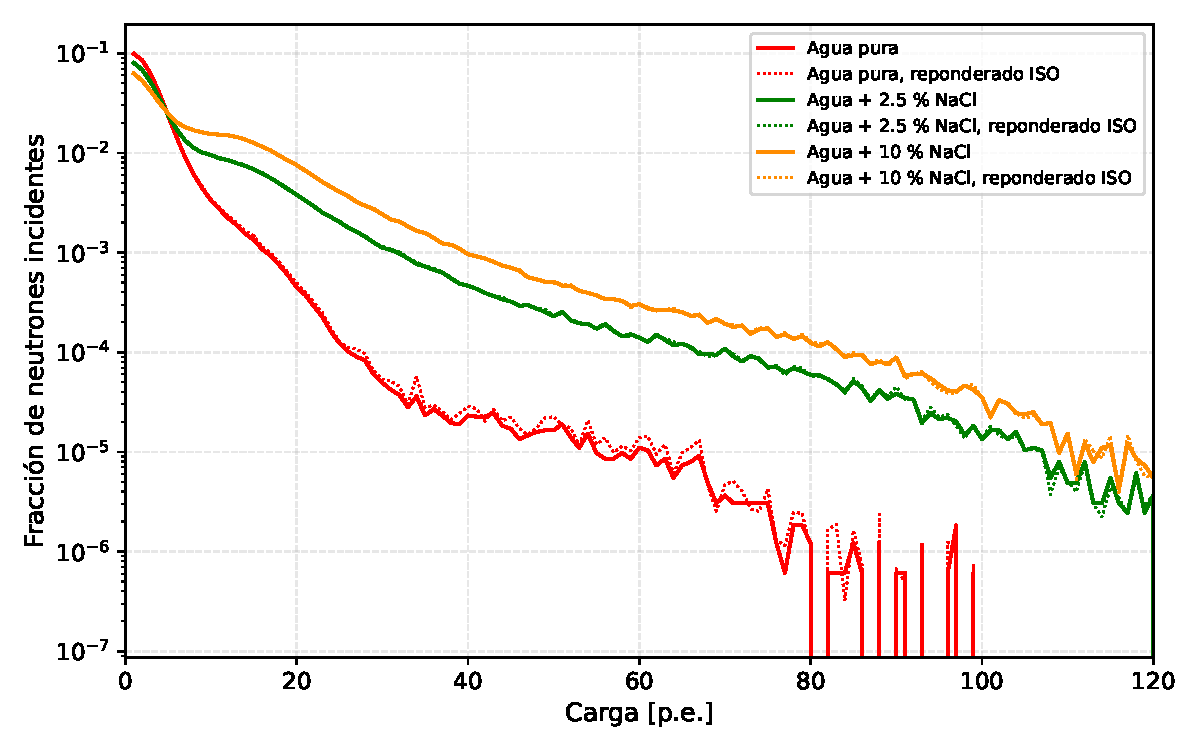
\includegraphics[width=0.7\linewidth]{fig02_histograma_carga.pdf}
\caption{Distribución de carga por neutrón incidente, sin reponderar y reponderada al ISO.}\label{fig:q}\end{figure}

\subsection{Captura en agua pura (estimada)}\label{sec:etapura}
Sin archivos de pasos, la fracción de eventos con captura del haz en agua pura se estima de dos formas:
(A) a partir de la eficiencia medida, $\varepsilon=P(s|c)\,\eta+P(s|\bar c)(1-\eta)$, con $P(s|\bar c)$ de 2.5\,\% y
$P(s|c)$ de la Campaña~1 corregida por el cociente Am-Be/Campaña~1 de 2.5\,\%: $\eta=59.4$\,\%; (B) escalando la
$\eta$ de 2.5\,\% con el cociente agua pura/2.5\,\% de la Campaña~1: $\eta=54.3$\,\%. Se adopta
$\eta_\text{cap}=(56.9\pm2.6)$\,\%.

\section{Escalado al montaje blindado}
\paragraph{Método.} Para cada componente $c$ y observable $X$ (eventos con señal, capturas, carga total),
$N_X=N_c\,\langle X\rangle_c$:
\begin{itemize}
\item Haz (130\,711 n): $\langle X\rangle$ de las corridas Am-Be reponderadas al ISO.
\item Halo (167\,963 n, 0.5~eV--100~keV, $1/E$) y fondo (74\,598 n, $10^{-4}$--0.5~eV, maxwelliano a $kT=25.3$~meV): respuesta de la Campaña~1 (16 energías, 100\,000 neutrones cada una, misma inyección por la tapa) promediada con el espectro de la componente, con interpolación lineal en $\log E$ y valor constante fuera de la malla (1~meV--1~keV). Por encima de 1~keV la respuesta es casi plana, así que la extrapolación hasta 100~keV cambia los resultados menos del 1\,\%. Los medios de la Campaña~1 que se usan son agua pura, 2.5\,\% y 10\,\%.
\end{itemize}

\begin{table}[H]\centering\footnotesize\setlength{\tabcolsep}{3pt}\caption{Respuesta de la Campaña 1 promediada con el espectro de cada componente (por neutrón incidente).}\label{tab:c1}
\begin{tabular}{llccccc}\toprule
Medio & Componente & $\varepsilon(Q\geq1)$ [\%] & $\eta_\text{cap}$ [\%] & $P(s|c)$ [\%] & $\langle Q|Q\geq1\rangle$ & $\varepsilon(Q\geq20)$ [\%] \\\midrule
Agua pura & Halo (0.5 eV--100 keV, $1/E$) & 17.72 & 34.59 & 51.2 & 3.17 & 0.038 \\
Agua pura & Fondo ($10^{-4}$--0.5 eV, Maxwell) & 14.61 & 30.11 & 48.5 & 3.20 & 0.033 \\
\addlinespace
Agua + 2.5\,\% NaCl & Halo (0.5 eV--100 keV, $1/E$) & 22.51 & 39.03 & 57.7 & 7.47 & 1.947 \\
Agua + 2.5\,\% NaCl & Fondo ($10^{-4}$--0.5 eV, Maxwell) & 19.24 & 34.95 & 55.0 & 7.46 & 1.653 \\
\addlinespace
Agua + 10\,\% NaCl & Halo (0.5 eV--100 keV, $1/E$) & 30.34 & 47.90 & 63.4 & 10.58 & 4.500 \\
Agua + 10\,\% NaCl & Fondo ($10^{-4}$--0.5 eV, Maxwell) & 27.57 & 45.72 & 60.3 & 10.47 & 4.044 \\
\bottomrule\end{tabular}\end{table}

\begin{table}[H]\centering\footnotesize
\caption{Escalado a los 373\,272 neutrones que entran al tanque en 5~min (1~Ci, montaje blindado). $^\dagger$Captura del haz en agua pura estimada.}\label{tab:esc}
\setlength{\tabcolsep}{2.5pt}
\begin{tabular}{llrrrrrrr}\toprule
Medio & Comp. & $N$ & $\varepsilon$ [\%] & Señal ($Q\geq1$) & Capturas & $\langle Q\rangle$ [p.e.] & Carga total [p.e.] & $Q\geq20$ \\\midrule
Agua pura & Haz & 130\,711 & 36.4 & 47\,627 & 74\,310$^\dagger$ & 3.54 & 168\,555 & 395 \\
 & Halo & 167\,963 & 17.7 & 29\,765 & 58\,104 & 3.17 & 94\,501 & 63 \\
 & Fondo & 74\,598 & 14.6 & 10\,895 & 22\,463 & 3.20 & 34\,815 & 24 \\
 & \textbf{Total} & 373\,272 & 23.7 & \textbf{88\,287} & 154\,877$^\dagger$ & 3.37 & \textbf{297\,872} & 483 \\
\midrule
Agua + 2.5\,\% NaCl & Haz & 130\,711 & 42.2 & 55\,103 & 80\,064 & 7.79 & 429\,520 & 5\,173 \\
 & Halo & 167\,963 & 22.5 & 37\,806 & 65\,555 & 7.47 & 282\,339 & 3\,271 \\
 & Fondo & 74\,598 & 19.2 & 14\,350 & 26\,072 & 7.46 & 107\,038 & 1\,233 \\
 & \textbf{Total} & 373\,272 & 28.7 & \textbf{107\,258} & 171\,691 & 7.63 & \textbf{818\,897} & 9\,676 \\
\midrule
Agua + 10\,\% NaCl & Haz & 130\,711 & 49.4 & 64\,545 & 86\,479 & 11.16 & 720\,305 & 10\,548 \\
 & Halo & 167\,963 & 30.3 & 50\,955 & 80\,462 & 10.58 & 539\,175 & 7\,558 \\
 & Fondo & 74\,598 & 27.6 & 20\,566 & 34\,103 & 10.47 & 215\,306 & 3\,017 \\
 & \textbf{Total} & 373\,272 & 36.5 & \textbf{136\,065} & 201\,044 & 10.84 & \textbf{1\,474\,786} & 21\,122 \\
\bottomrule\end{tabular}\end{table}

\begin{figure}[H]\centering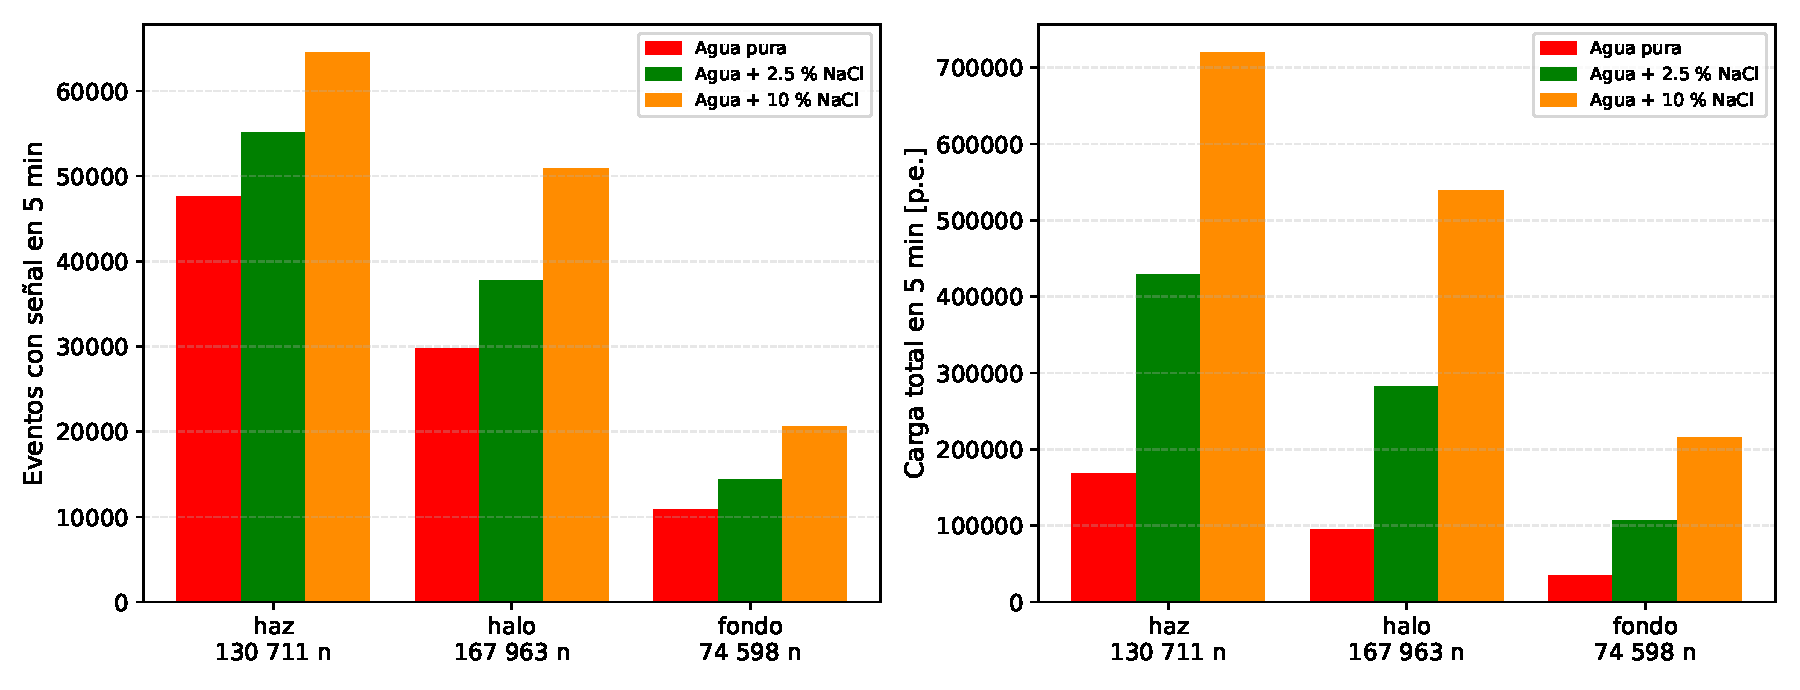
\includegraphics[width=\linewidth]{fig05_escalado_componentes.pdf}
\caption{Eventos con señal y carga total en 5~min por componente.}\label{fig:esc}\end{figure}

\paragraph{Resultado.} En 5 minutos se esperan 88\,287, 107\,258 y 136\,065
eventos con señal (294, 358 y 454~s$^{-1}$). Frente a agua pura, el NaCl multiplica los eventos
con señal por 1.21 (2.5\,\%) y 1.54 (10\,\%), la carga total por 2.75 y 4.95, y los eventos con
$Q\geq20$~p.e. por 20 y 44. El haz aporta el 35\,\% de los neutrones, pero
47--54\,\% de las señales y 49--57\,\% de la carga, porque sus neutrones rápidos se capturan más
adentro. Las incertidumbres estadísticas son $\lesssim1$\,\%; dominan las sistemáticas del modelo.

\aviso{\textbf{Salvedades.} (1) Todas las corridas usadas inyectan los neutrones por la tapa,
mientras que el montaje real irradia por el costado a media altura. La geometría cambia la fracción que
escapa y, sobre todo, la carga, porque el PMT está en la tapa. Los valores absolutos son una
\emph{estimación}; los cocientes NaCl/agua pura son más robustos. (2) El haz no incluye la degradación
de energía al cruzar los 10~cm de plomo. (3) Las fracciones 35/45/20\,\% y la normalización
($T_\text{Pb}=0.313$) son hipótesis del modelo del montaje. (4) En agua pura la captura del haz está
estimada. (5) Las corridas no usan S($\alpha,\beta$), igual que la Campaña~1. (6) MEIGA trata cada
neutrón como un evento aislado: a ~1\,200~n/s y $\tau\sim0.1$--0.2~ms, en el detector real se apilan unos
0.1--0.3 neutrones por ventana de captura. Para la cifra definitiva hay que correr en MEIGA el archivo de
373\,272 neutrones del montaje (inyección por el costado).}

\section{Histograma de carga y comparación con el detector prototipo}
\paragraph{Histograma simulado.} El archivo \archivo{histogramas_comparados.txt} que usa el notebook
\archivo{analisis-datos-Flujo-Completo-Bga.ipynb} (TOSHIBA, \archivo{Detector-prototipo/Nuevo-analisis/})
es \emph{exactamente} el histograma de carga de las tres corridas Am-Be (bins de 1~p.e., 591\,639 / 685\,718 / 804\,279 eventos con $Q\geq1$).
Para el montaje de 5~min se construyó el histograma esperado
$h_\text{5min}=130\,711\,h_\text{haz}^\text{ISO}+167\,963\,h_\text{halo}+74\,598\,h_\text{fondo}$, con los histogramas de la
Campaña~1 plegados con el espectro de cada componente (\archivo{resultados/histograma_carga_simulado.tsv}, Fig.~\ref{fig:hsim}).

\begin{figure}[H]\centering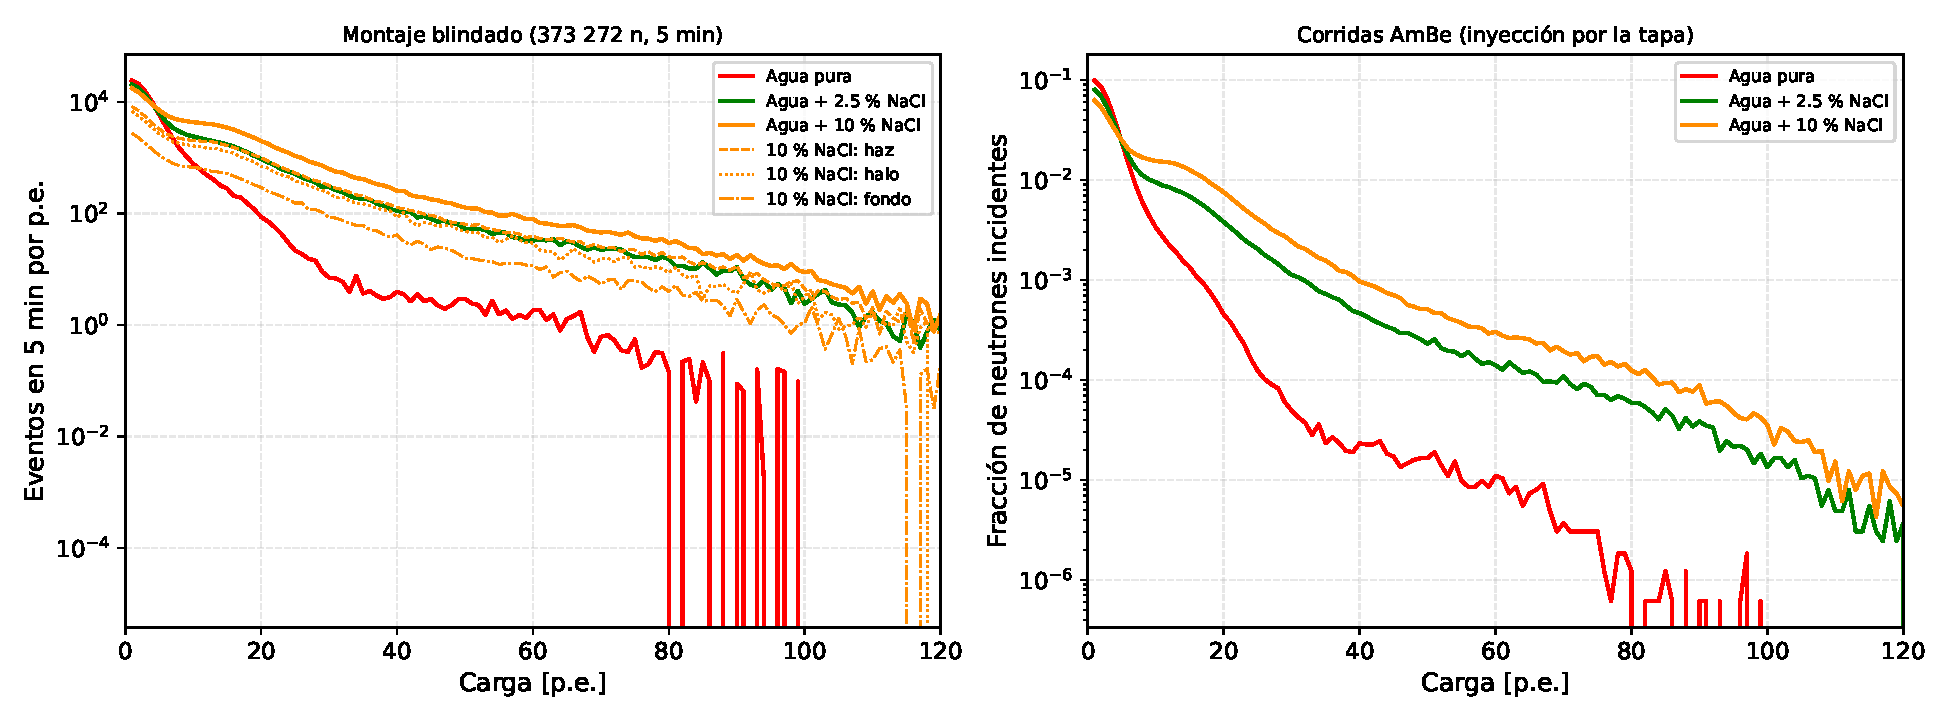
\includegraphics[width=\linewidth]{fig07_histograma_carga_simulado.pdf}
\caption{Histograma de carga simulado. Izquierda: montaje blindado en 5~min, con el desglose por componente para 10\,\% NaCl. Derecha: corridas Am-Be por neutrón incidente.}\label{fig:hsim}\end{figure}

\paragraph{Datos experimentales.} Seis tomas LAGO (fuente + fondo y fondo, por medio). La carga por pulso se calculó con el
mismo algoritmo del notebook: traza de 32 muestras, ventana positiva que contiene la muestra 8, pico $>1200$~ADC y suma de la
ventana. Se reproducen exactamente sus conteos (por ejemplo, agua pura: 194\,459 y 79\,682 pulsos). Datos de cada toma:
\begin{center}\small\begin{tabular}{lcccccc}\toprule
 & \multicolumn{2}{c}{Agua pura} & \multicolumn{2}{c}{2.5\,\% NaCl} & \multicolumn{2}{c}{10\,\% NaCl} \\
 & fuente & fondo & fuente & fondo & fuente & fondo \\\midrule
Duración [s] & 300 & 300 & 300 & 299 & 240 & 299 \\
Pulsos con carga & 194\,459 & 79\,682 & 663\,709 & 88\,827 & 1\,875\,731 & 145\,522 \\
Umbral T1 [ADC] & \multicolumn{2}{c}{800} & \multicolumn{2}{c}{1000} & \multicolumn{2}{c}{1080} \\
HV leído [V] & 827 & 813 & 830 & 828 & 878 & 877 \\
Pico de muones del fondo [p.e.] & \multicolumn{2}{c}{162} & \multicolumn{2}{c}{154} & \multicolumn{2}{c}{154} \\
\bottomrule\end{tabular}\end{center}

\aviso{\textbf{Observaciones sobre el notebook.} (1) La toma con fuente en 10\,\% dura 240~s y su fondo 299~s, pero el notebook
resta los conteos sin normalizar por tiempo. Aquí la resta es $(h_n/t_n-h_f/t_f)\times300$~s; en este caso el efecto es pequeño
(1.6\,\%), porque la fuente domina. (2) En el notebook la simulación se multiplica por un factor arbitrario de 0.3 y el agua pura
se desplaza $-1500$~ADC; aquí se usa la normalización absoluta. (3) El umbral de disparo y la HV cambian entre medios, pero el
pico de muones del fondo cae en el mismo sitio (154--162~p.e., $\pm5$\,\%), así que la calibración de 3.95~p.e. por 1000~ADC
vale para los tres medios.}

\begin{figure}[H]\centering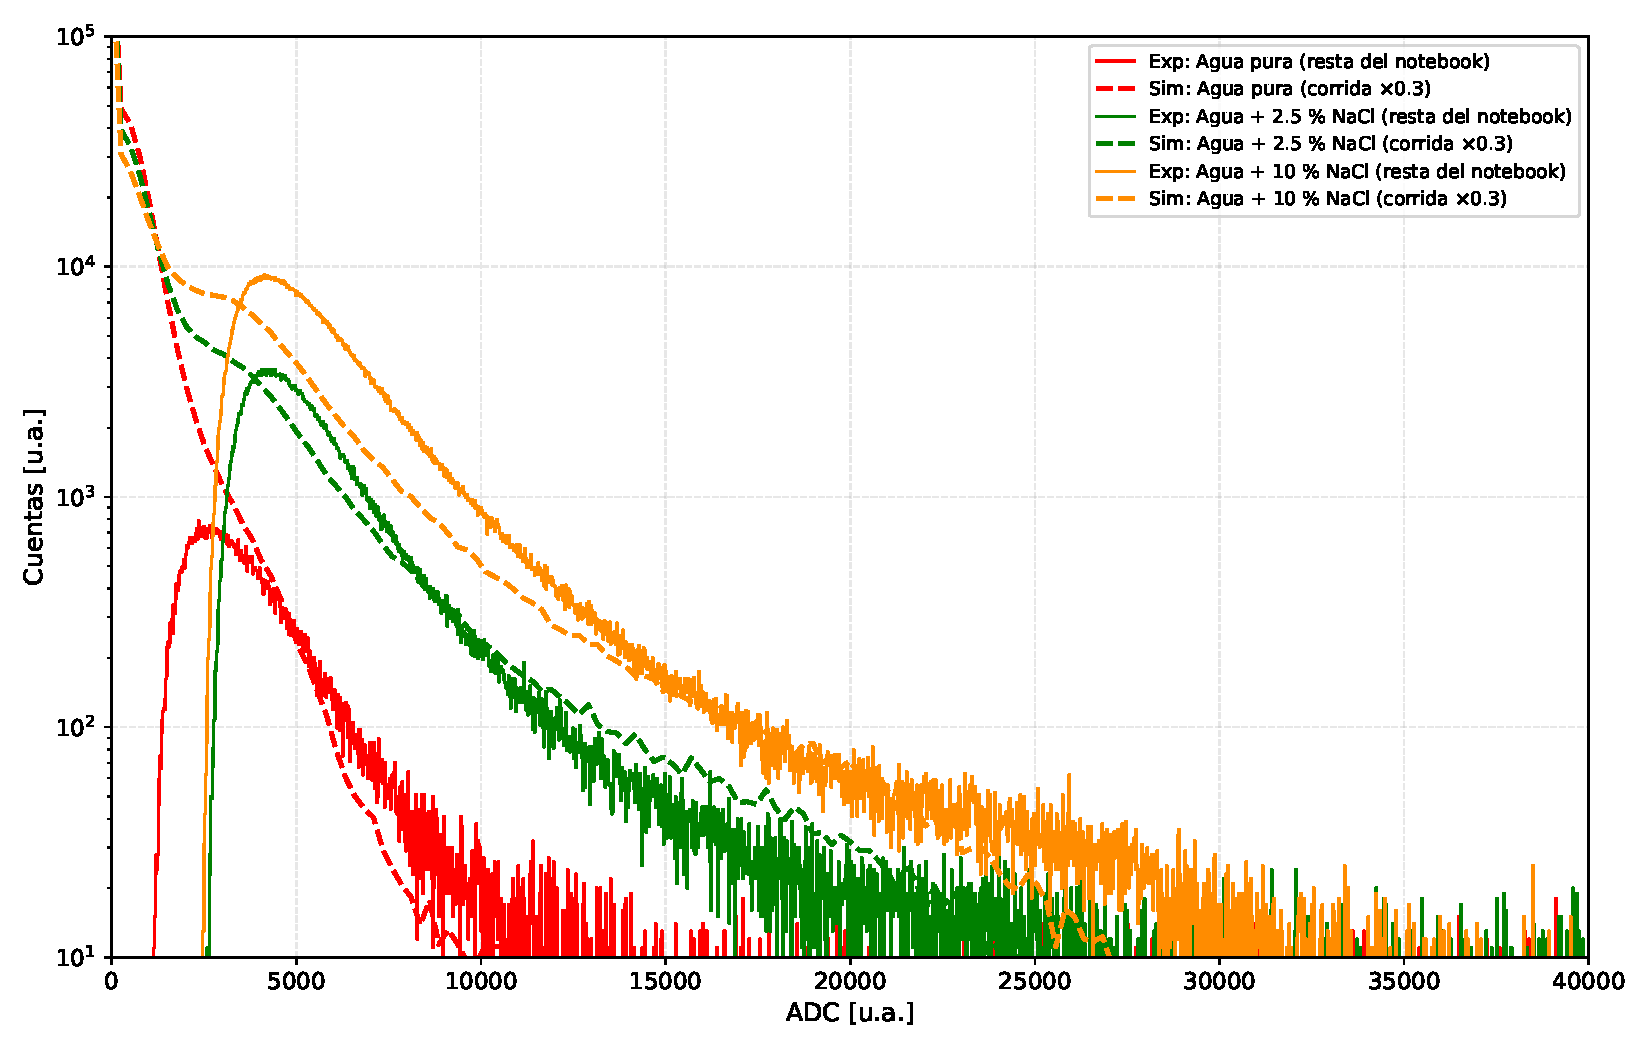
\includegraphics[width=0.78\linewidth]{fig09_reproduccion_notebook.pdf}
\caption{Reproducción de la figura del notebook: ADC, simulación de la corrida $\times0.3$, agua pura desplazada $-1500$~ADC.}\label{fig:nb}\end{figure}
\begin{figure}[H]\centering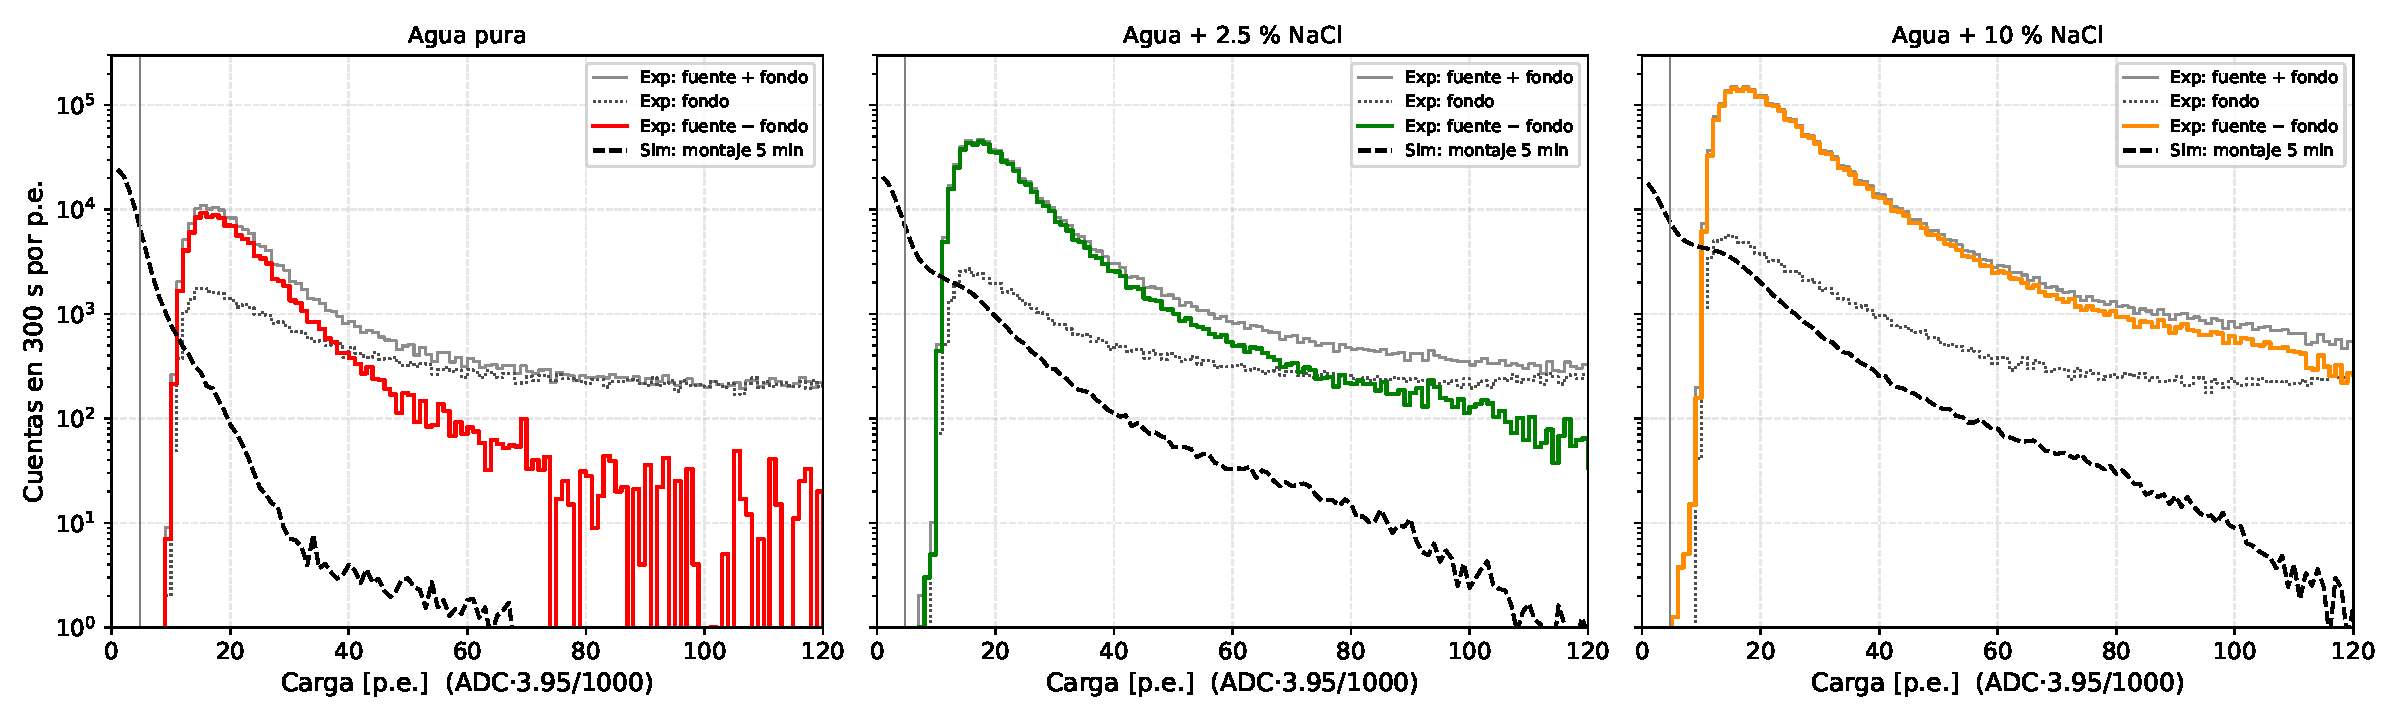
\includegraphics[width=\linewidth]{fig08_experimento_vs_simulacion.pdf}
\caption{Experimento (fuente, fondo y fuente $-$ fondo normalizado a 300~s) frente a la simulación del montaje de 5~min, en p.e. La línea vertical marca el corte de 1200~ADC.}\label{fig:exp}\end{figure}
\begin{figure}[H]\centering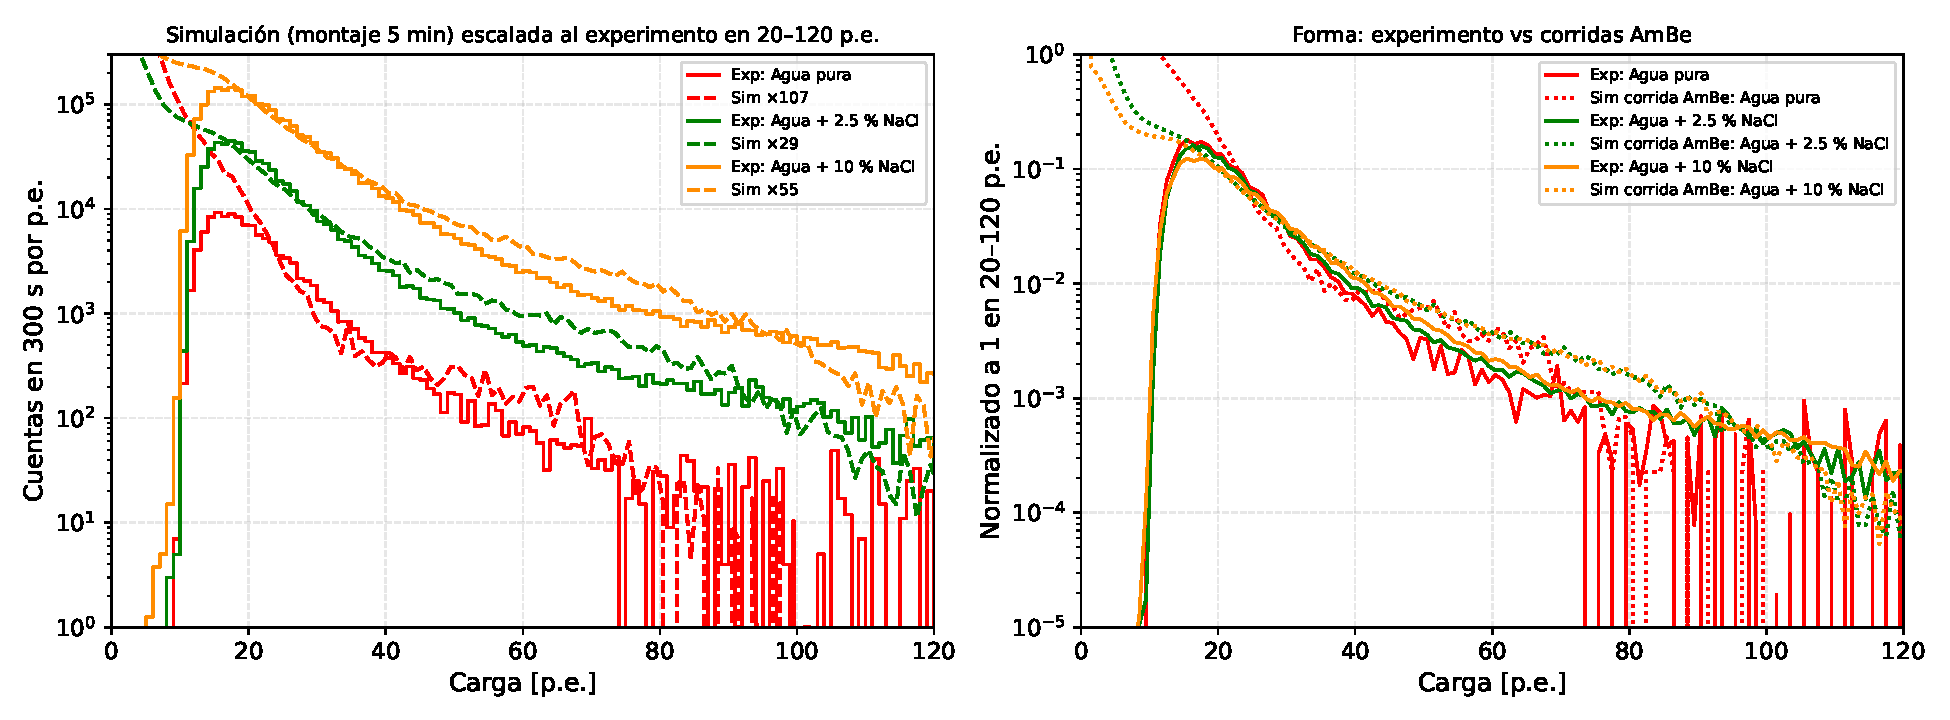
\includegraphics[width=\linewidth]{fig10_forma_exp_vs_sim.pdf}
\caption{Izquierda: simulación del montaje escalada al experimento en 20--120~p.e. Derecha: comparación de forma (normalizada en 20--120~p.e.).}\label{fig:forma}\end{figure}

\begin{table}[H]\centering\small\caption{Cuentas netas en 5~min por encima de un umbral de carga: experimento frente a la simulación del montaje.}\label{tab:exp}
\begin{tabular}{lccc}\toprule
 & Agua pura & 2.5\,\% NaCl & 10\,\% NaCl \\\midrule
Exp. neto, $Q\geq10$~p.e. & 114\,770 & 574\,576 & 2\,198\,474 \\
Sim. montaje, $Q\geq10$~p.e. & 4\,038 & 27\,294 & 55\,690 \\
Exp./Sim. ($Q\geq10$) & 28 & 21 & 39 \\
Exp. neto, $Q\geq20$~p.e. & 52\,345 & 282\,848 & 1\,173\,777 \\
Neutrones incidentes equivalentes ($Q\geq10$) & 10.6\,M (1.6\,\%) & 7.9\,M (1.2\,\%) & 14.7\,M (2.2\,\%) \\
\bottomrule\end{tabular}\end{table}

\paragraph{Resultados.}
\begin{enumerate}
\item \textbf{Normalización absoluta.} Por encima de 10~p.e. el experimento tiene 28 / 21 / 39 veces más cuentas netas que el
montaje modelado (373\,272 neutrones). Para reproducirlas harían falta ${\sim}$8--15~millones de neutrones incidentes en 5~min,
es decir, el 1.2--2.2\,\% de lo que emite 1~Ci, frente al 0.056\,\% del modelo blindado (y el 30\,\% de la fuente desnuda). O bien
el blindaje real deja pasar unas 20--40 veces más neutrones que el modelo, o la actividad o la geometría de la fuente son otras.
\item \textbf{Forma.} En 2.5\,\% y 10\,\% NaCl la forma simulada sigue a la experimental entre 20 y 60~p.e. (Fig.~\ref{fig:forma}).
En agua pura la simulación cae mucho más rápido que el experimento: el espectro experimental de agua pura tiene casi la misma
forma que el de NaCl. Eso apunta a una componente de la señal experimental que no depende del medio y que la simulación no
incluye, por ejemplo los gammas de 4.44~MeV de la fuente que atraviesan el plomo, o neutrones rápidos que entran por el costado.
\item \textbf{Efecto del NaCl.} Las cuentas netas con $Q\geq20$~p.e. crecen $\times$5.4 (2.5\,\%) y $\times$22.4 (10\,\%) en el experimento,
frente a $\times$20 y $\times$44 en la simulación. El signo y el orden se reproducen; la magnitud no, en parte por el exceso
de señal en agua pura del punto anterior.
\item Por debajo de ${\sim}12$~p.e. no se puede comparar: el corte de 1200~ADC en el pico elimina los pulsos pequeños del experimento.
\end{enumerate}

\section{Histogramas sin fondo y número de neutrones por medio}
\paragraph{Origen.} Las curvas ``sin fondo'' del autor están en
\archivo{Detector-prototipo/Comparacion-robusta-fondo-neutrones-\{agua-pura, A25NaCl, agua-10NaCl\}/Diferencia-datos-A-*.dat}.
Método: para cada disparo, la línea base es la mediana de las 20 primeras muestras y la carga es la suma de la parte positiva de
las 32 muestras; se cuentan todos los disparos, sin corte; 6000 bins entre 10 y 60\,000~ADC; diferencia = fuente $-$ fondo.
\archivo{scripts/histogramas_sin_fondo.py} (con \archivo{scripts/carga_robusta.awk}) reproduce los tres archivos
\textbf{exactamente} (diferencia 0 en todos los bins, Fig.~\ref{fig:sf1}). La curva original de 10\,\% corresponde a 240~s de
fuente menos 299~s de fondo; aquí las tres se normalizan por tiempo a 300~s (Fig.~\ref{fig:sf2}).

\begin{figure}[H]\centering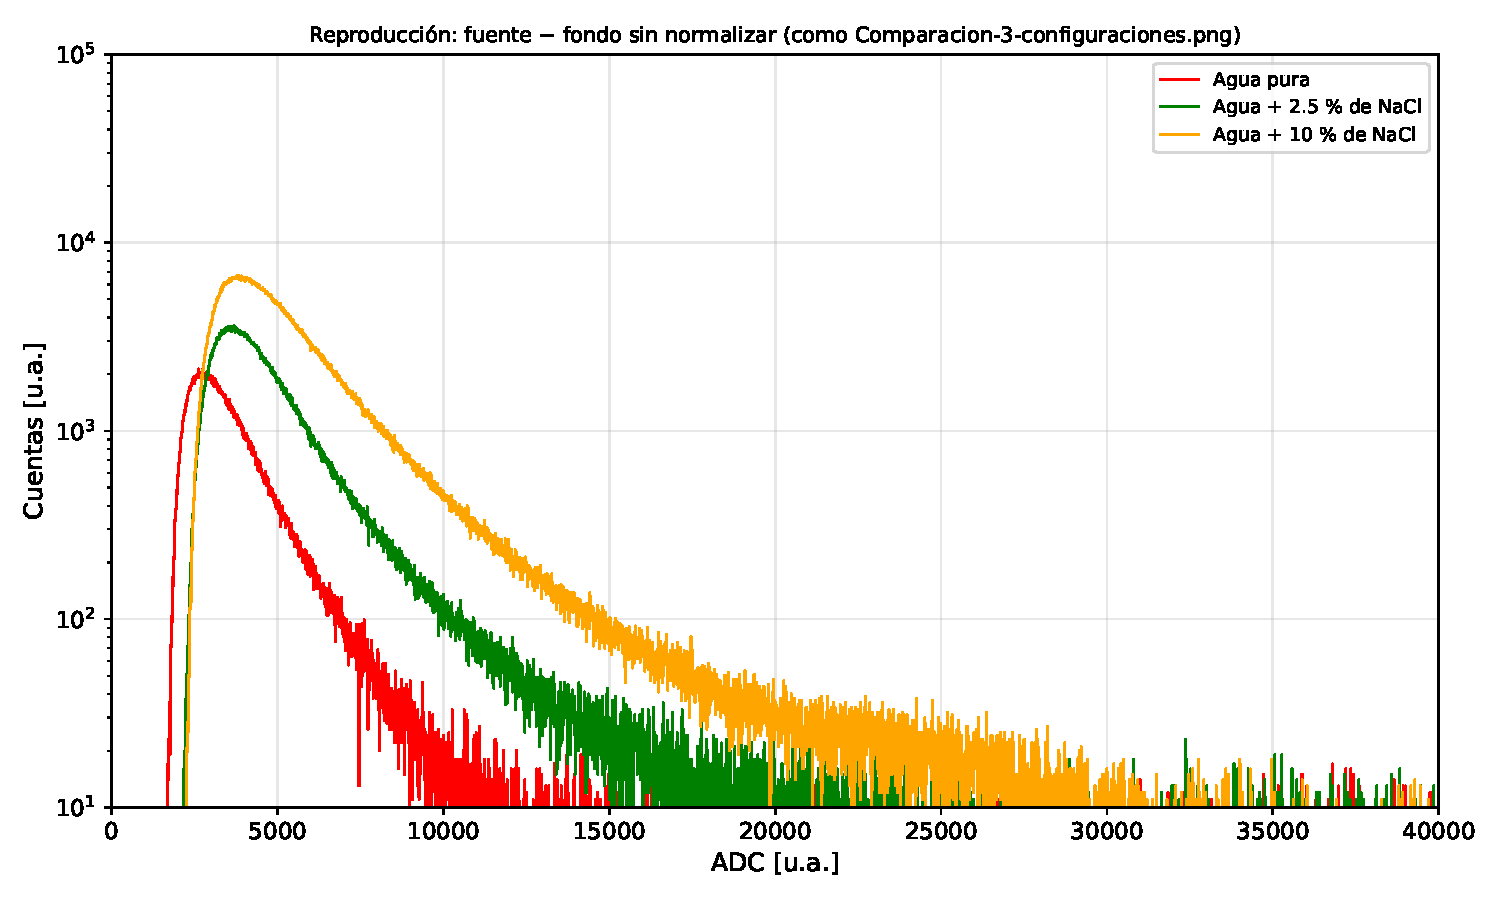
\includegraphics[width=0.75\linewidth]{fig11_sin_fondo_reproduccion.pdf}
\caption{Reproducción de los histogramas sin fondo del autor (fuente $-$ fondo sin normalizar, en ADC).}\label{fig:sf1}\end{figure}
\begin{figure}[H]\centering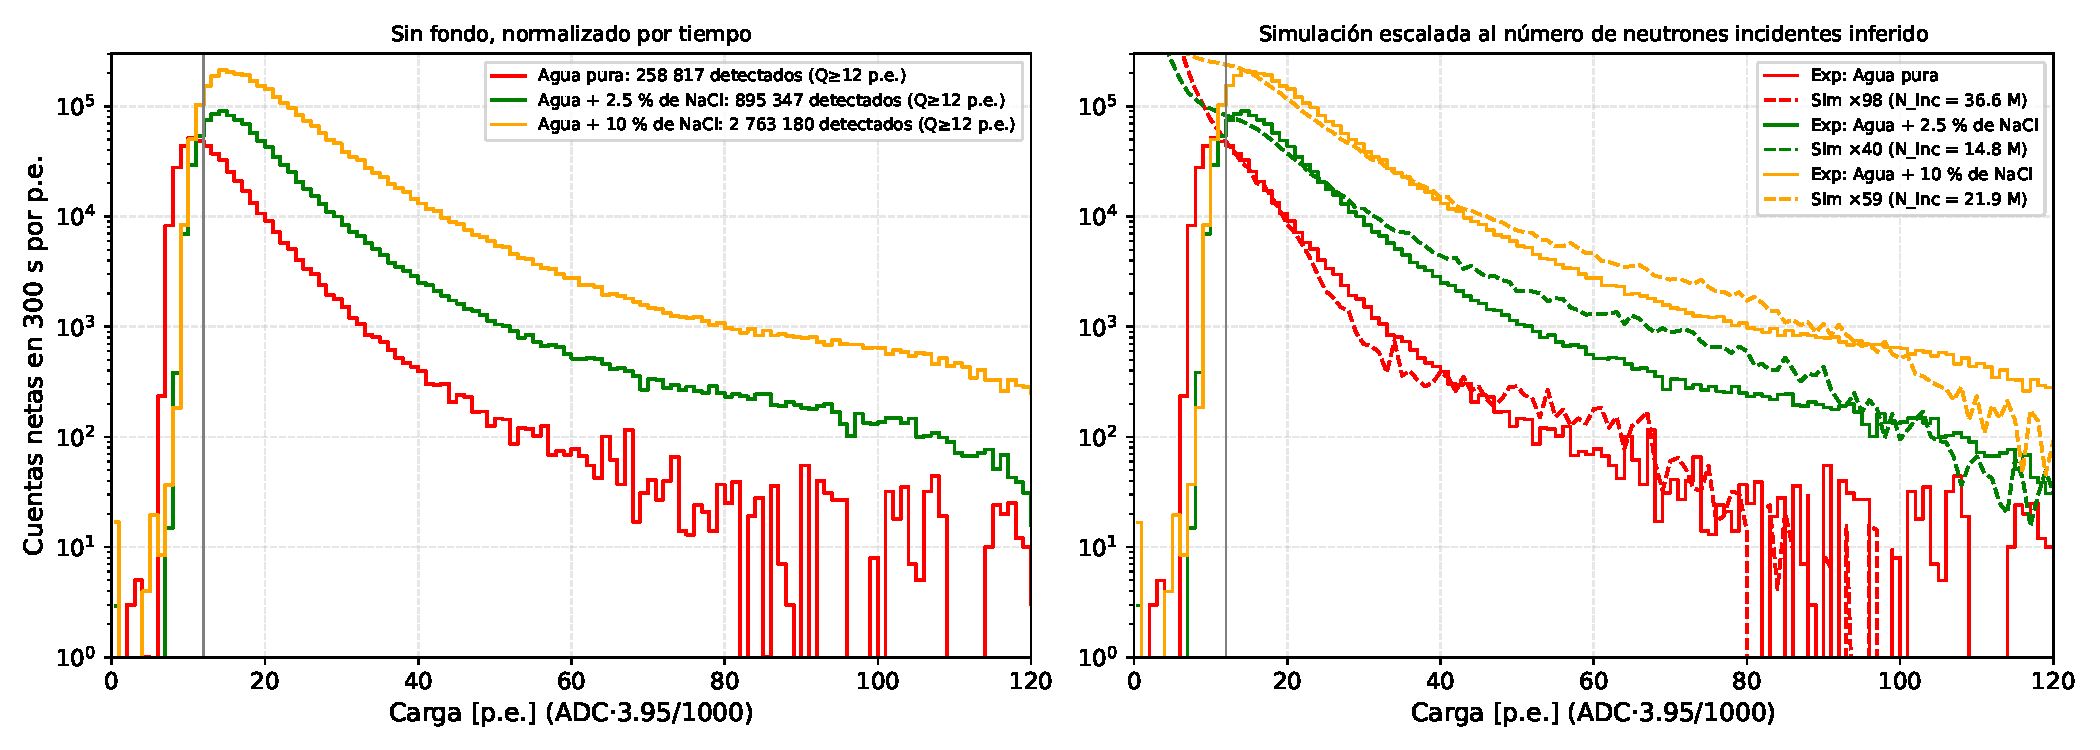
\includegraphics[width=\linewidth]{fig12_sin_fondo_normalizado.pdf}
\caption{Izquierda: histogramas sin fondo normalizados a 300~s, en p.e. Derecha: simulación del montaje escalada al número de neutrones incidentes inferido para cada medio. La línea vertical marca el umbral de 12~p.e.}\label{fig:sf2}\end{figure}

\paragraph{Neutrones por medio.} Detectados = pulsos netos con $Q\geq12$~p.e., por encima del codo de disparo de los tres medios.
Incidentes = detectados / eficiencia simulada por neutrón incidente (respuesta del montaje: haz + halo + fondo).
Capturados = incidentes $\times$ capturas por neutrón simuladas.
\begin{table}[H]\centering\small\caption{Neutrones en 5~min (300~s) por medio, a partir de los histogramas sin fondo.}\label{tab:sf}
\begin{tabular}{lccc}\toprule
 & Agua pura & 2.5\,\% NaCl & 10\,\% NaCl \\\midrule
Disparos netos totales (sin umbral) & 438\,560 & 985\,079 & 2\,924\,148 \\
\textbf{Detectados} ($Q\geq12$ p.e.) & \textbf{258\,817} & \textbf{895\,347} & \textbf{2\,763\,180} \\
Tasa de detección [s$^{-1}$] & 863 & 2\,984 & 9\,211 \\
Eficiencia simulada por neutrón incidente [\%] & 0.71 & 6.07 & 12.62 \\
\textbf{Incidentes (insertados)} & \textbf{36.6\,M} & \textbf{14.8\,M} & \textbf{21.9\,M} \\
\quad\% de lo emitido por 1~Ci & 5.5 & 2.2 & 3.3 \\
\textbf{Capturados} & \textbf{15.2\,M} & \textbf{6.8\,M} & \textbf{11.8\,M} \\
Detectados con captura & 231\,993 (90\,\%) & 885\,179 (99\,\%) & 2\,749\,002 (99\,\%) \\
Carga media detectados: medida / simulada [p.e.] & 18.2 / 17.0 & 20.6 / 22.5 & 23.2 / 23.0 \\
Pico de muones del fondo [p.e.] & 154 & 138 & 146 \\
\bottomrule\end{tabular}\end{table}

\paragraph{Interpretación.}
\begin{itemize}
\item \textbf{Forma.} Con este método la forma del espectro coincide con la simulación en los tres medios, también en agua pura
(la carga media difiere menos del 10\,\%). Casi toda la señal detectada viene de capturas: 90\,\% en agua pura y 99\,\% con NaCl.
\item \textbf{Número de incidentes.} Con la misma fuente, el número de neutrones que entran al tanque debería ser igual en los tres
medios, pero sale 36.6 / 14.8 / 21.9~M. Si cada medio se calibra con su propio pico de
muones, los valores cambian menos del 7\,\%, así que la diferencia no se debe a la calibración. Las tomas son de fechas distintas,
con otro umbral y otra HV: es posible que la geometría o la posición de la fuente hayan cambiado. En agua pura puede contribuir
además una señal de la fuente que no es captura de neutrones (gammas de 4.44~MeV).
\item \textbf{Valor absoluto.} Entran entre 15 y 37 millones de neutrones en 5~min (2--5\,\% de 1~Ci), 40--100 veces más que los
373\,272 del modelo blindado: el blindaje real deja pasar muchos más neutrones de lo supuesto.
\end{itemize}

\section{Conclusiones}
\begin{enumerate}
\item Las tres corridas Am-Be (1\,637\,458 neutrones cada una) están completas y se recuperaron con el CRC verificado. En agua pura solo se conservan la carga por evento y los archivos procesados de gammas y electrones.
\item Reponderar al espectro ISO cambia la eficiencia y la carga menos del 2\,\% relativo: los resultados anteriores con el archivo sesgado siguen siendo válidos para estos observables.
\item El NaCl aumenta la eficiencia por neutrón ($\times$1.36 al 10\,\%) y, sobre todo, las señales grandes ($\times$27 en $Q\geq20$), gracias a la captura en $^{35}$Cl.
\item Escalado al montaje blindado (373\,272 neutrones en 5~min): 88\,287 / 107\,258 / 136\,065 eventos con señal y
297\,872 / 818\,897 / 1\,474\,786~p.e. de carga total (agua pura / 2.5\,\% / 10\,\%), con la salvedad de la inyección por la tapa.
\item Histogramas sin fondo del prototipo (5~min, $Q\geq12$~p.e.): 258\,817 / 895\,347 / 2\,763\,180 neutrones detectados, 36.6 / 14.8 / 21.9~M incidentes y 15.2 / 6.8 / 11.8~M capturados (agua pura / 2.5\,\% / 10\,\%). La forma coincide con la simulación; el número de incidentes no es el mismo en los tres medios.
\end{enumerate}
\end{document}
